\section{Kartézský souřadnicový systém}
\label{appendix:vektorova_analyza}

Složky libovolného vektoru jsou v~obecném případě funkcí souřadnic a~času. Nejprve ukážeme tvary operátorů v~kartézském souřadnicovém systému $x, y, z$ s~příslušnými jednotkovými vektory $\mathbf{i}$, $\mathbf{j}$ a~$\mathbf{k}$.

\begin{figure}[!hbt]
\centering
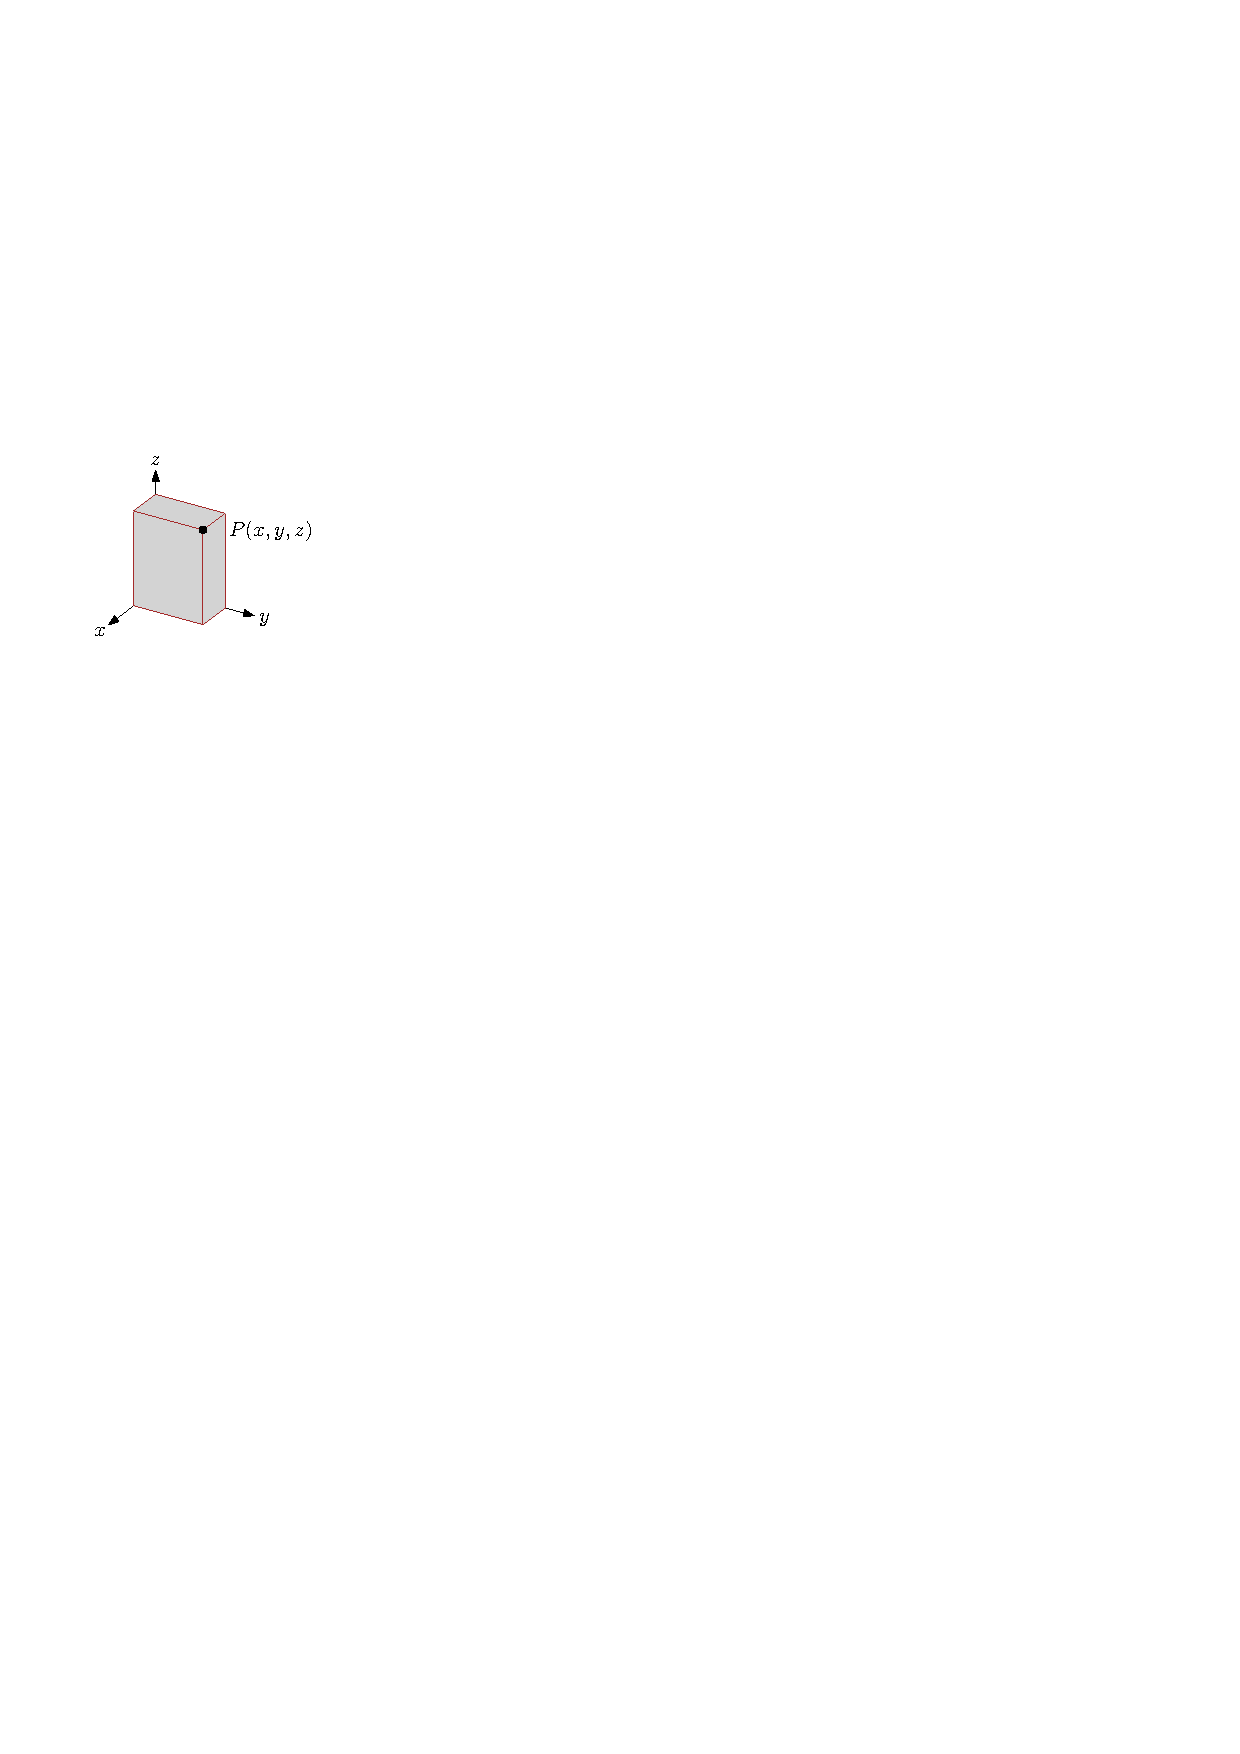
\includegraphics[]{prilohy/vektorova_analyza/kartezsky.pdf}
\caption{Kartézský souřadnicový systém}
\label{fig:vektorova_analyza_kartezsky}
\end{figure}

Zavedeme operátor „nabla“ -- $\nabla$, který je definován jako
$$
\nabla = \mathbf{i}\,\frac{\partial}{\partial x} + \mathbf{j}\,\frac{\partial}{\partial y} + \mathbf{k}\,\frac{\partial}{\partial z}\,.
$$
Pomocí tohoto operátoru lze jednoduše nadefinovat všechny tři důležité diferenciální operátory: gradient, divergenci a~rotaci.

\subsection*{Gradient}

Gradient skalární funkce $\varphi$ lze vyjádřit ve tvaru
$$
\grad \varphi = \nabla\varphi\ = \mathbf{i}\,\frac{\partial \varphi}{\partial x} + \mathbf{j}\,\frac{\partial \varphi}{\partial y} + \mathbf{k}\,\frac{\partial \varphi}{\partial z}\,.
$$

\subsection*{Divergence}

Divergence vektorového pole $\vec A(x, y, z)$ zapíšeme jako

$$
\div \vec A = \nabla \cdot \vec A = \frac{\partial A_x}{\partial x} + \frac{\partial A_y}{\partial y} + \frac{\partial A_z}{\partial z}
$$
kde $A_x$, $A_y$ a~$A_z$ jsou složky vektorové funkce $\vec A(x, y, z)$.

\subsection*{Rotace}

Rotaci vektorového pole $\vec A(x, y, z)$ definujeme výrazem
$$
\vec A = \nabla \times \vec A = 
\left|
\begin{array}{ccc}
  \mathbf{i} & \mathbf{j} & \mathbf{k} \\
  \frac{\partial}{\partial x} & \frac{\partial}{\partial y} & \frac{\partial}{\partial z} \\
  A_x & A_y & A_z
\end{array}
\right|\,.
$$

\subsection*{Laplaceův operátor}

Operátor $\nabla^2$ (nebo také $\triangle$) se nazývá Laplaceův operátor a~lze vyjádřit ve tvaru
$$
\nabla^2 = \triangle = \frac{\partial^2}{\partial x^2}+\frac{\partial^2}{\partial y^2}+
\frac{\partial^2}{\partial z^2}.
$$
Může působit na skalární nebo vektorovou funkci
$$
\nabla^2 \varphi = \triangle \varphi = \frac{\partial^2\varphi}{\partial x^2}+\frac{\partial^2\varphi}{\partial y^2}+
\frac{\partial^2\varphi}{\partial z^2},
$$
$$
\triangle\, \vec A = \frac{\partial^2 \vec A}{\partial x^2} + \frac{\partial^2 \vec A}{\partial y^2} + 
\frac{\partial^2 \vec A}{\partial z^2}.
$$
Laplaceův operátor splňuje Laplaceovu rovnici. 

\subsection*{Operátor rot rot}

Jeden z~často používaných operátorů je rot rot. V~případě kartézského systému souřadnice je snadné odvodit vztah
$$
\rot \rot \vec A = \grad \div \vec A - \triangle\,\vec A.
$$

\section{Válcový souřadnicový systém}

Válcový souřadnicový systém je definován vztahy
$$
x = r\cos \alpha,\ \ y = r \sin \alpha,\ \ z = z,\ \ \alpha \in \langle 0,2\pi \rangle.
$$

\begin{figure}[!hbt]
\centering
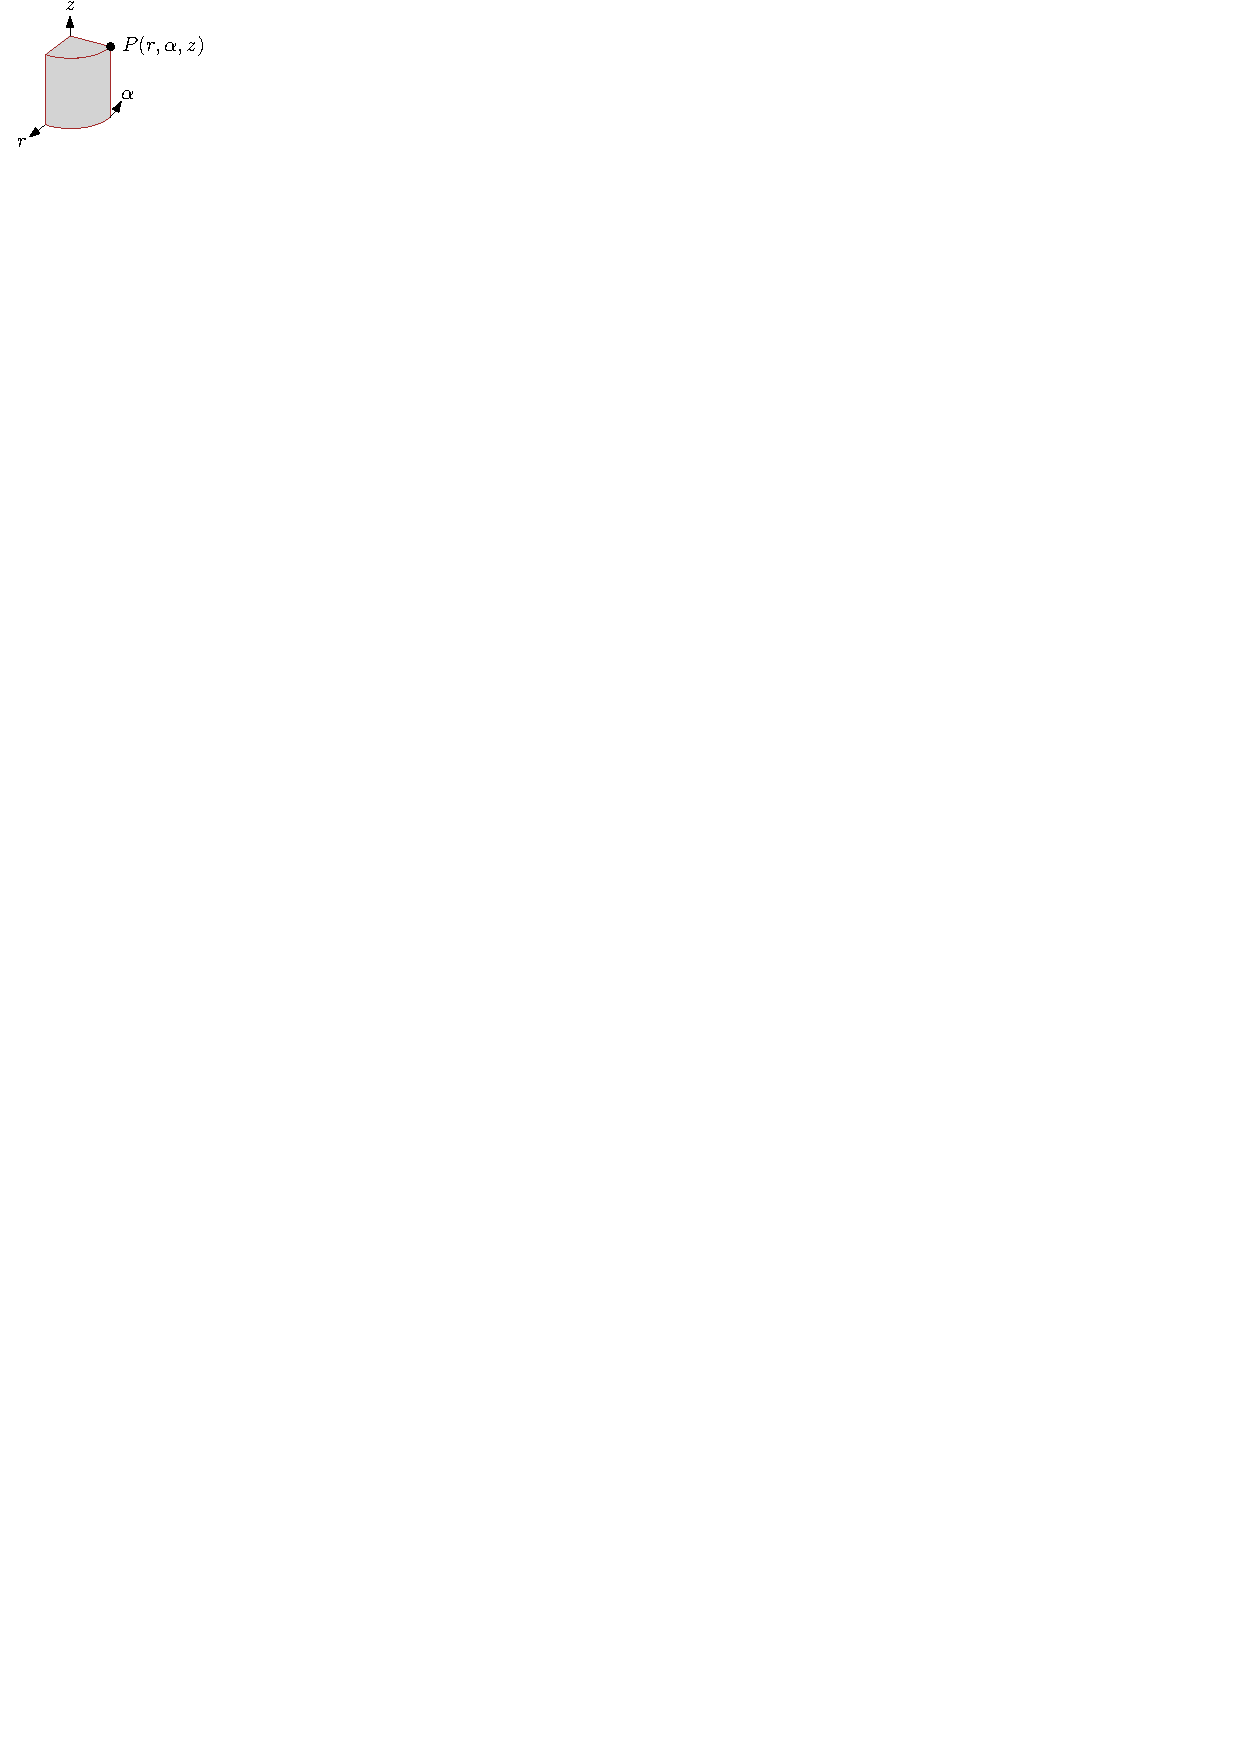
\includegraphics[]{prilohy/vektorova_analyza/valcovy.pdf}
\caption{Válcový souřadnicový systém}
\label{fig:vektorova_analyza_valcovy}
\end{figure}

Příslušné diferenciální operátory gradient, divergence a~rotace lze za použití jednotkových vektorů $\textbf{r}_0$, $\textbf{a}_0$ a~$\textbf{z}_0$ zapsat ve tvaru
$$
\grad \,\varphi=\mbox{\textbf{r}}_0 \frac{\partial\varphi}{\partial r}
+\mbox{\textbf{a}}_0\frac{1}{r}\frac{\partial\varphi}{\partial \alpha}+
\mbox{\textbf{z}}_0\frac{\partial\varphi}{\partial z},
$$
$$
\div \vec A = \frac{1}{r}\frac{\partial (rA_r)}{\partial r}+
\frac{1}{r}\frac{\partial A_\alpha}{\partial \alpha}+\frac{\partial A_z}{\partial z} = 
\frac{\partial A_r}{\partial r} + \frac{A_r}{r} +
\frac{1}{r}\frac{\partial A_\alpha}{\partial \alpha}+\frac{\partial A_z}{\partial z},
$$
$$
\rot \vec A = \frac{1}{r}\cdot
\left|
\begin{array}{ccc}
  \mbox{\textbf{r}}_0 & r\mbox{\textbf{a}}_0 & \mbox{\textbf{z}}_0 \\
  \frac{\partial}{\partial r} & \frac{\partial}{\partial \alpha} & \frac{\partial}{\partial z} \\
  A_r & rA_\alpha & A_z
\end{array}
\right|
$$
a~$$
\triangle = \frac{1}{r}\frac{\partial}{\partial r}\left(r
\frac{\partial}{\partial r}\right) + \frac{1}{r^2}\frac{\partial^2}{\partial \alpha^2} + \frac{\partial^2}{\partial z^2}.
$$
Mnohem komplikovanější (s~ohledem na kartézský systém) je zápis operátoru rot rot. Po několika úpravách dostaneme
$$
\rot \rot \vec A = \mbox{\textbf{r}}_0\left[-\frac{1}{r^2}\frac{\partial^2 A_r}
{\partial \alpha^2}-\frac{\partial^2 A_r}{\partial z^2}+\frac{1}{r^2}\frac{\partial A_\alpha}
{\partial \alpha}+\frac{1}{r}\frac{\partial^2 A_\alpha}{\partial r\partial \alpha}+
\frac{\partial^2 A_z}{\partial r \partial z}\right]+
$$
$$
+\,\mbox{\textbf{a}}_0\left[\frac{1}{r}\frac{\partial^2 A_r}
{\partial r \partial\alpha}-\frac{1}{r^2}\frac{\partial A_r}{\partial \alpha}-
\frac{\partial^2 A_\alpha}{\partial z^2}+\frac{A_\alpha}{r^2}-\frac{1}{r}\frac{\partial A_\alpha}
{\partial r}-\frac{\partial^2 A_\alpha}{\partial r^2}+\frac{1}{r}\frac{\partial^2 A_z}
{\partial \alpha \partial z}\right]+
$$
$$
+\,\mbox{\textbf{z}}_0\left[\frac{\partial^2 A_r}{\partial r \partial z}+\frac{1}{r}
\frac{\partial A_r}{\partial z}+\frac{1}{r}\frac{\partial^2 A_\alpha}{\partial \alpha \partial z}-
\frac{1}{r^2}\frac{\partial A_z}{\partial \alpha^2}-
\frac{\partial^2 A_z}{\partial r^2}-\frac{1}{r}\frac{\partial A_z}{\partial r}\right]\,.
$$

V~osově symetrických uspořádání se setkáme zpravidla se dvěma případy:

\begin{itemize}
\item Vektor $\vec A$ má pouze jedinou nenulovou složku $A_\alpha$ v~tangenciálním směru $\alpha$ a~tato složka závisí pouze na souřadnicích $r$ a~$z$. V~tomto případě má výsledný vektor také pouze jedinou nenulovou složku ve směru $\alpha$ a~je dán vztahem
$$
\rot \rot \vec A_\alpha =
\frac{A_\alpha}{r^2}-\frac{1}{r}\frac{\partial A_\alpha}{\partial r}-
\frac{\partial^2 A_\alpha}{\partial r^2}-\frac{\partial^2 A_\alpha}{\partial z^2}.
$$
\item Vektor $\vec A$ má pouze jedinou nenulovou složku $A_z$ v~axiálním směru $z$ a~tato složka závisí pouze na souřadnici $z$. V~tomto případě má výsledný vektor také pouze jedinou nenulovou složku ve směru $z$ a~je dán vztahem
$$
\rot \rot \vec A_z=-\frac{\partial^2 A_z}{\partial r^2}-
\frac{1}{r}\frac{\partial A_z}{\partial r}\,.
$$
\end{itemize}

\subsection*{Gaussova věta}

Gaussova věta určuje vztah mezi tokem vektorového pole uzavřenou plochou a~jeho chováním uvnitř této oblasti. Uvažujme objem $V$ obepínaný po částech spojitou uzavřenou plochou $\partial V$ a~vektorové pole $\vec A$ spojitě diferencovatelné na $V \cup \partial V$, pak platí vztah
$$
\int_V \div \vec A \dif V = \oint_{\partial V} \vec A \cdot \mathrm{n}_\mathrm{0} \dif S,
$$
kde $\mathrm{n}_\mathrm{0}$ značí jednotkový normálový vektor k~hranici $\partial V$. 

\subsection*{Stokesova věta}

Stokesova věta určuje vztah mezi cirkulací vektorového pole podél uzavřené křivky a~jeho chováním na ploše, kterou tato křivka obepíná. Uvažujme plochu $S$ obepínanou po částech spojitou křivkou $\partial S$ a~vektorové pole $\vec A$ spojitě diferencovatelné na $S \cup \partial S$, pak platí vztah
$$
\int_S \rot \vec A \cdot \dif S = \oint_{\partial S} \vec A \cdot \dif \vec l,
$$
kde $\dif \vec l$ je jednotkový vektor v~tečném směru ke křivce $\partial S$.



































%Vector analysis is one of the domains of mathematics that deals the
%differential and integral operations with vectors, generally in
%multidimensional spaces. It contains a lot of various rules and techniques
%that are very useful for solving a wide spectrum of physical and engineering
%problems. Vector analysis also provides efficient tools for treatment of different
%physical fields of both scalar and vector character.
%
%This section contains a brief summary of the terminology, definitions and
%fundamental rules in the domain. The most important formulae are expressed
%both in the Cartesian and cylindrical coordinate systems that are mostly used for
%solving technical tasks discussed throughout this book.
%
%\subsection{Differential and integral operations with vectors in Cartesian coordinates}
%
%As was mentioned in the previous section, the components of any vector may generally
%be functions of time and/or space (in the simplest case, however, they are
%constants). We start with the relevant vector operations in the
%Cartesian coordinate system $x,y,z$ with unit vectors $\mathbf{i}$, $\mathbf{j}$
%and $\mathbf{k}$.
%
%Let us first introduce a formal vector operator $\nabla$ called ``nabla'' (or ``del'') that is
%defined as follows
%$$
%\nabla=\mathbf{i}\,\frac{\partial}{\partial x}+\mathbf{j}\,\frac{\partial}{\partial
%y}+\mathbf{k}\,\frac{\partial}{\partial z}\,.
%$$
%This operator is of great importance for defining three fundamental differential
%operators \inxx{differential, operator} grad, div and curl.
%
%\subsubsection{Gradient}
%
%The {\it gradient} \inxx{gradient} of a scalar function $\varphi(x,y,z)$ is a vector defined as
%$$
%\grad \,\varphi=\mathbf{i}\,\frac{\partial \varphi}{\partial x}+\mathbf{j}\,
%\frac{\partial \varphi}{\partial y}+\mathbf{k}\,\frac{\partial \varphi}{\partial z}\,.
%$$
%At a given point this vector shows the direction of the maximum change in a scalar
%field. The operator grad can evidently also be written in terms of the
%operator ``nabla''
%$$
%\grad \,\varphi=\nabla\varphi\,.
%$$
%
%\subsubsection{Divergence}
%
%The {\it divergence} \inxx{divergence} of a vector function $\mbox{\vec p}(x,y,z)$ is a scalar
%defined as
%$$
%\mbox{div {\vec p}}=\frac{\partial A_x}{\partial x}+\frac{\partial A_y}{\partial y}+
%\frac{\partial A_z}{\partial z}
%$$
%where $A_x$, $A_y$ and $A_z$ are individual components of the vector {\vec p}.
%At a given point it provides the magnitude of the source or sink of the
%vector field. The operator div can similarly be written in terms of the
%operator ``nabla''
%$$
%\mbox{div {\vec p}}=\nabla\cdot\mbox{\vec p}\,.
%$$
%
%\subsubsection{Circulation}
%
%The {\it circulation} \inxx{circulation} of a vector function $\mbox{\vec p}(x,y,z)$ is a vector
%defined as
%$$
%\mbox{curl {\vec p}}=
%\left|
%\begin{array}{ccc}
%  \mathbf{i} & \mathbf{j} & \mathbf{k} \\
%  \frac{\partial}{\partial x} & \frac{\partial}{\partial y} & \frac{\partial}{\partial z} \\
%  A_x & A_y & A_z
%\end{array}
%\right|\,.
%$$
%At a given point of a vector field this operator shows the tendency of the vector {\vec p} to
%rotate about it. Even here we can use the operator ``nabla'' for definition
%$$
%\mbox{curl {\vec p}}=\nabla\times\mbox{\vec p}\,.
%$$
%
%\subsubsection{Connectedness}
%
%Connectedness \inxx{connectedness} is an important topological property used for distinguishing
%topological spaces. A topological space is called connected (or simply-connected)
%if it cannot be represented by a disjoint union of two and more nonempty open subsets.
%It is clear from Fig. \ref{fig:vect_anal} that shows an example of a connected
%subset (part a) and a not connected subset (part b).
%
%\begin{figure}[h]
%\centering
%\includegraphics[width=8 cm]{A12/Connect}
%\caption{To the connectedness of a domain.}
%\label{fig:vect_anal}
%\end{figure}
%
%A stronger requirement is on a path-connected space, which is a domain where
%any two points $A$ and $B$ can be connected by a path lying in this domain (part a),
%which is impossible in part b).
%
%\subsubsection{Conservative vector fields}
%
%Every vector field that is given by the gradient of a scalar function is
%called conservative. So that the vector field $\mbox{\vec p}$ defined by
%$$
%\mbox{\vec p}=\grad \,\varphi
%$$
%is conservative.
%
%Consider now integral
%$$
%I=\int_A^B\mbox{\vec p}\cdot\dif \mbox{\vec r}
%$$
%where $\mbox{\vec r}=(x,y,z)$ is the position vector, so that $\dif\mbox{\vec r}=
%(\dif x,\dif y,\dif z)$ and $A$ and $B$ are two arbitrary points. The expression can
%be rewritten as
%$$
%I=\int_A^B \grad \,\varphi\cdot\dif \mbox{\vec r}=\int_A^B \left(\frac{\partial
%\varphi}{\partial x},\frac{\partial \varphi}{\partial y},
%\frac{\partial \varphi}{\partial z}\right)(\dif x,\dif y,\dif z)=
%$$
%$$
%\int_A^B \left(\frac{\partial \varphi}{\partial x}\dif x+\frac{\partial \varphi}{\partial y}\dif y+
%\frac{\partial \varphi}{\partial z}\dif z\right)=\int_A^B \dif
%\varphi=\varphi(B)-\varphi(A).
%$$
%It is clear that the integral is absolutely independent of the path, it just
%depends on its endpoints. Hence, for any closed loop $\rm c$
%$$
%\oint_{\rm c} \mbox{\vec p}\cdot\dif \mbox{\vec r}=0.
%$$
%The converse is true, however, only when the domain containing the path $\rm c$ is a connected
%region.
%
%\subsubsection{Irrotational vector fields}
%
%A vector field $\mbox{\vec p}$ is called irrotational \inxx{irrotational, vector field}
%(or curl-free) if
%$$
%\nabla\mbox{\vec p}=\mbox{\textbf{0}}.
%$$
%It may easily be shown that for any scalar function $\varphi$
%$$
%\nabla\times\nabla\,\varphi=\mbox{\textbf{0}},
%$$
%which leads to the conclusion that any conservative field \inxx{conservative, field} is also an
%irrotational field. The converse of this statement is true if the domain is again
%simply-connected.
%
%\subsubsection{Solenoidal vector fields}
%
%Every vector field $\mbox{\vec p}$ whose divergence is equal to zero is called
%solenoidal \inxx{solenoidal, field}. This condition is satisfied if
%\begin{equation}
%\mbox{\vec p}=\rot \,\mbox{\vec A}
%\label{eq:vectan1}
%\end{equation}
%(it can easily be shown that for any vector function {\vec A} div(curl\,{\vec A})=0). The converse also holds:
%if a vector field $\mbox{\vec p}$ is solenoidal, there always exist a vector function
%{\vec A} satisfying (\ref{eq:vectan1}).
%
%\subsubsection{Laplacian vector fields}
%
%Every vector field $\mbox{\vec p}$ that is irrotational and sole\-noidal is called the
%Laplacian vector field \inxx{Laplacian, vector, field}. This field also satisfies conditions
%$$
%\rot \,\mbox{\vec p}=\mbox{\textbf{0}},
%$$
%$$
%\div \,\mbox{\vec p}=0.
%$$
%Thus, the vector field $\mbox{\vec p}$ may be expressed as grad$\,\varphi$ and
%the last equation can be rewritten as
%$$
%\nabla\cdot\nabla\,\varphi=\nabla^2\,\varphi=\triangle\varphi=0.
%$$
%The operator $\nabla^2$ is called the Laplacian operator and we denote it
%also by symbol $\triangle$. Normally we write it in the form
%$$
%\triangle=\frac{\partial^2}{\partial x^2}+\frac{\partial^2}{\partial y^2}+
%\frac{\partial^2}{\partial z^2}
%$$
%and it may act on both scalar and vector functions, so that
%$$
%\triangle \varphi=\frac{\partial^2\varphi}{\partial x^2}+\frac{\partial^2\varphi}{\partial y^2}+
%\frac{\partial^2\varphi}{\partial z^2},
%$$
%$$
%\triangle\, \mbox{\vec p}=\frac{\partial^2\mbox{\vec p}}{\partial x^2}+\frac{\partial^2\mbox{\vec p}}
%{\partial y^2}+\frac{\partial^2\mbox{\vec p}}{\partial z^2}.
%$$
%The Laplacian operator satisfies Laplace's equation.
%
%\subsubsection{Operator curl\,curl}
%
%One of the frequently used operators is also operator curl\,curl. In the
%Cartesian coordinate system it can easily be shown that
%$$
%\mbox{curl\,curl {\vec p}}=\mbox{grad\,div {\vec p}}-\triangle\,\mbox{\vec p}\,.
%$$
%
%\subsubsection{Gauss' theorem (or divergence theorem)}
%
%This theorem \inxx{Gauss, theorem} provides a relation between a flow of a vector field through a
%closed surface to its behavior in the volume inside it. Consider a 3D compact domain
%$V$ with a piecewise smooth boundary $\partial V$. If $\mbox{\vec p}$ is a vector field
%continuously differentiable in $V \cup \partial V$, then
%$$
%\int_V(\nabla\cdot\mbox{\vec p})\dif V=\oint_{\partial V}(\mbox{\vec p}\cdot\mbox{\tu
%n}_0)\dif S
%$$
%where $\mbox{\vec n}_0$ denotes the outward unit normal to the boundary $\partial V$.
%While the left-hand side of the above equation represents the total source of vector
%$\mbox{\vec p}$ in volume $V$, the right-hand side gives the total flow from
%the volume $V$ through its boundary $\partial V$.
%
%\subsubsection{Stokes' theorem}
%
%This theorem \inxx{Stokes, theorem} provides a relation between the circulation of a vector field
%along a piecewise smooth simple closed path to its behavior on the area bounded by this path.
%Consider a 2D domain $S$ with a piecewise smooth path $\partial S$. If $\mbox{\vec p}$ is a vector
%field continuously differentiable in $S \cup \partial S$, then
%$$
%\int_S(\nabla\times\mbox{\vec p})\dif S=\oint_{\partial S}(\mbox{\vec p}\cdot\dif \mbox{\tu
%l})
%$$
%where $\dif \mbox{\vec l}$ is the elementary vector in the tangential direction
%to the path $\partial S$.
%
%\subsubsection{Green's theorem}
%
%This theorem represents Stokes' theorem in 2D \inxx{Green, theorem}. Consider a positively
%oriented simple closed curve $C$ in plane $x,y$ that is piecewise smooth. Let $S$ be the
%domain bounded by $C$. If $f(x,y)$ and $g(x,y)$ are continuously differentiable
%functions defined on $S$, then
%$$
%\oint_C\left(f(x,y)\dif x+g(x,y)\dif y\right)=
%\int_S\left(\frac{\partial g(x,y)}{\partial x}-\frac{\partial f(x,y)}{\partial y}\right)\dif S.
%$$
%
%\subsection{Other orthogonal coordinate systems}
%
%The versatility of the vector calculus is based on the fact that the form of vector
%equations does not depend on the coordinate system. But particular computations are
%mostly realized using the component equations, in such a system that allows for their
%easiest solution. Therefore, it is very useful to know the transformation rules
%for the components of various vectors in different systems and also for
%various vector operators.
%
%Consider a Cartesian coordinate system $(x,y,z)$ and continuous functions $u(x,y,z)$,
%$v(x,y,z)$ and $w(x,y,z)$ that are also continuously differentiable except for
%a finite number of points. These functions may be called curvilinear coordinates
%\inxx{curvilinear, coordinates}.
%
%Let $P$ is an arbitrary point and {\vec r} its position vector. In the curvilinear
%system $u,v,w$ its elementary change is described by vector
%$$
%\dif \mbox{\vec r}=\frac{\partial \mbox{\vec r}}{\partial u}\,\dif u+
%\frac{\partial \mbox{\vec r}}{\partial v}\,\dif v+
%\frac{\partial \mbox{\vec r}}{\partial w}\,\dif w\,.
%$$
%Vectors
%$$
%\mbox{\vec a}_1=\frac{\partial \mbox{\vec r}}{\partial u},
%\mbox{\vec a}_2=\frac{\partial \mbox{\vec r}}{\partial v},
%\mbox{\vec a}_3=\frac{\partial \mbox{\vec r}}{\partial w}
%$$
%are called the basic vectors (but not necessarily of unit magnitude) at point $P$ and
%the only condition they should satisfy is their linear independence. In such a case they
%form at point $P$ the fundamental coordinate system. If the curvilinear
%system is orthogonal \inxx{orthogonal, system}, the basic vectors are perpendicular to each other.
%
%\subsubsection{Metric coefficients in orthogonal systems}
%
%In the Cartesian coordinate system the elementary shift is given by relation
%$$
%\dif s=\sqrt{(\dif x)^2+(\dif y)^2+(\dif z)^2}
%$$
%where, for instance, $\dif x$ may be expressed (using the curvilinear
%coordinates) as
%$$
%\dif x=\frac{\partial x}{\partial u}\,\dif u+
%\frac{\partial x}{\partial v}\,\dif v+
%\frac{\partial x}{\partial w}\,\dif w\,,
%$$
%and analogously we can express $\dif y$ and $\dif z$. Now we can write
%$$
%\dif s=\sqrt{(\dif u,\dif v, \dif w)\cdot
%\begin{pmatrix}
%  g_{11} & g_{12} & g_{13} \\
%  g_{21} & g_{22} & g_{23} \\
%  g_{31} & g_{32} & g_{33}
%\end{pmatrix}
%\cdot
%\begin{pmatrix}
%  \dif u \\
%  \dif v \\
%  \dif w
%\end{pmatrix}
%}
%$$
%where elements $g_{11},\ldots,g_{33}$ are called metric coefficients defined
%by relations \inxx{metric, coefficients}
%$$
%g_{11}=\frac{\partial x}{\partial u}\cdot\frac{\partial x}{\partial u}+
%\frac{\partial y}{\partial u}\cdot\frac{\partial y}{\partial u}+
%\frac{\partial z}{\partial u}\cdot\frac{\partial z}{\partial u},
%$$
%$$
%g_{12}=g_{21}=\frac{\partial x}{\partial u}\cdot\frac{\partial x}{\partial v}+
%\frac{\partial y}{\partial u}\cdot\frac{\partial y}{\partial v}+
%\frac{\partial z}{\partial u}\cdot\frac{\partial z}{\partial v},
%$$
%$$
%g_{13}=g_{31}=\frac{\partial x}{\partial u}\cdot\frac{\partial x}{\partial w}+
%\frac{\partial y}{\partial u}\cdot\frac{\partial y}{\partial w}+
%\frac{\partial z}{\partial u}\cdot\frac{\partial z}{\partial w},
%$$
%$$
%g_{22}=\frac{\partial x}{\partial v}\cdot\frac{\partial x}{\partial v}+
%\frac{\partial y}{\partial v}\cdot\frac{\partial y}{\partial v}+
%\frac{\partial z}{\partial v}\cdot\frac{\partial z}{\partial v},
%$$
%$$
%g_{23}=g_{32}=\frac{\partial x}{\partial v}\cdot\frac{\partial x}{\partial w}+
%\frac{\partial y}{\partial v}\cdot\frac{\partial y}{\partial w}+
%\frac{\partial z}{\partial v}\cdot\frac{\partial z}{\partial w},
%$$
%$$
%g_{33}=\frac{\partial x}{\partial w}\cdot\frac{\partial x}{\partial w}+
%\frac{\partial y}{\partial w}\cdot\frac{\partial y}{\partial w}+
%\frac{\partial z}{\partial w}\cdot\frac{\partial z}{\partial w}.
%$$
%
%If the curvilinear coordinate system is orthogonal, the elements
%$$
%g_{12}=g_{21}=g_{13}=g_{31}=g_{23}=g_{32}=0,
%$$
%so that
%\begin{equation}
%\dif s=\sqrt{g_{11}(\dif u)^2+g_{22}(\dif v)^2+g_{33}(\dif w)^2}.
%\label{eq:metrics1}
%\end{equation}
%Putting
%\begin{equation}
%h_1=\sqrt{g_{11}},\ \ h_2=\sqrt{g_{22}},\ \ h_3=\sqrt{g_{33}}
%\label{eq:metrics2}
%\end{equation}
%and the element (\ref{eq:metrics1}) can be rewritten into the form
%$$
%\dif s=\sqrt{(h_1\dif u)^2+(h_2\dif v)^2+(h_3\dif w)^2}.
%$$
%The quantities $h_1,\ h_2$ and $h_3$ are called Lam\'e coefficients
%\inxx{Lam\'e, coefficients}.
%
%\subsubsection{Vector operators in orthogonal systems}
%
%The gradient of a scalar function $\varphi$ is given by formula
%$$
%\grad \,\varphi=\mbox{\textbf{u}}_1 \frac{1}{h_1}\frac{\partial\varphi}{\partial u}
%+\mbox{\textbf{u}}_2\frac{1}{h_2}\frac{\partial\varphi}{\partial v}+
%\mbox{\textbf{u}}_3\frac{1}{h_3}\frac{\partial\varphi}{\partial w}\,.
%$$
%where $\mbox{\textbf{u}}_1$, $\mbox{\textbf{u}}_2$ and $\mbox{\textbf{u}}_3$
%are the unit vectors in the directions specified by the individual orthogonal
%directions.
%
%The divergence of a vector function {\vec p} has the form
%$$
%\mbox{div \vec p}=\frac{1}{h_1h_2h_3}\left[\frac{\partial (h_2h_3A_1)}{\partial u}+
%\frac{\partial (h_1h_3A_2)}{\partial v}+\frac{\partial (h_1h_2A_3)}{\partial w}\right]
%$$
%where $A_1$, $A_2$ and $A_3$ are the components of the vector {\vec p} in the
%orthogonal directions.
%
%The circulation of a vector function {\vec p} is
%$$
%\mbox{curl \vec p}=\frac{1}{h_1h_2h_3}\cdot
%\left|
%\begin{array}{ccc}
%  h_1\mbox{\textbf{u}}_1 & h_2\mbox{\textbf{u}}_2 & h_3\mbox{\textbf{u}}_3 \\
%  \frac{\partial}{\partial u} & \frac{\partial}{\partial v} & \frac{\partial}{\partial w} \\
%  h_1A_1 & h_2A_2 & h_3A_3
%\end{array}
%\right|
%$$
%and finally Laplace's operator
%$$
%\triangle=\frac{1}{h_1h_2h_3}\cdot\left[\frac{\partial}{\partial u}\left(\frac{h_2h_3}{h_1}
%\frac{\partial}{\partial u}\right)+\frac{\partial}{\partial v}\left(\frac{h_3h_1}{h_2}
%\frac{\partial}{\partial v}\right)+\frac{\partial}{\partial w}\left(\frac{h_1h_2}{h_3}
%\frac{\partial}{\partial w}\right)\right].
%$$
%
%\subsubsection{Cylindrical coordinates}
%
%The cylindrical coordinates are defined by relations
%$$
%x=r\cos\alpha,\ \ y=r\sin\alpha,\ \ z=z,\ \ \alpha\in\langle 0,2\pi\rangle.
%$$
%From (\ref{eq:metrics2}) we immediately obtain
%$$
%h_1=1,\ \ h_2=r,\ \ h_3=1.
%$$
%
%\begin{figure}[h]
%\centering
%\includegraphics[width=8 cm]{A12/Cylcoor}
%\caption{To the determination of the cylindrical coordinates of point $P$.}
%\label{fig:cylinder}
%\end{figure}
%
%Denoting the unit vectors (see Fig. \ref{fig:cylinder}) in the directions of particular
%orthogonal axes as $\mbox{\textbf{r}}_0$, $\mbox{\textbf{a}}_0$ and $\mbox{\textbf{z}}_0$
%we get
%$$
%\grad \,\varphi=\mbox{\textbf{r}}_0 \frac{\partial\varphi}{\partial r}
%+\mbox{\textbf{a}}_0\frac{1}{r}\frac{\partial\varphi}{\partial \alpha}+
%\mbox{\textbf{z}}_0\frac{\partial\varphi}{\partial z}\,,
%$$
%$$
%\mbox{div \vec p}=\frac{1}{r}\frac{\partial (rA_r)}{\partial r}+
%\frac{1}{r}\frac{\partial A_\alpha}{\partial \alpha}+\frac{\partial A_z}{\partial z}\,,
%$$
%$$
%\mbox{curl \vec p}=\frac{1}{r}\cdot
%\left|
%\begin{array}{ccc}
%  \mbox{\textbf{r}}_0 & r\mbox{\textbf{a}}_0 & \mbox{\textbf{z}}_0 \\
%  \frac{\partial}{\partial r} & \frac{\partial}{\partial \alpha} & \frac{\partial}{\partial z} \\
%  A_r & rA_\alpha & A_z
%\end{array}
%\right|
%$$
%and
%$$
%\triangle=\frac{1}{r}\frac{\partial}{\partial r}\left(r
%\frac{\partial}{\partial r}\right)+\frac{1}{r^2}\frac{\partial^2}{\partial
%\alpha^2}+\frac{\partial^2}{\partial
%z^2}.
%$$
%
%Of a more complicated form (unlike the Cartesian coordinate system) is the operator curl\,curl.
%After some manipulation we obtain
%$$
%\mbox{curl\,curl\,{\vec p}}=\mbox{\textbf{r}}_0\left[-\frac{1}{r^2}\frac{\partial^2 A_r}
%{\partial \alpha^2}-\frac{\partial^2 A_r}{\partial z^2}+\frac{1}{r^2}\frac{\partial A_\alpha}
%{\partial \alpha}+\frac{1}{r}\frac{\partial^2 A_\alpha}{\partial r\partial \alpha}+
%\frac{\partial^2 A_z}{\partial r \partial z}\right]+
%$$
%$$
%+\,\mbox{\textbf{a}}_0\left[\frac{1}{r}\frac{\partial^2 A_r}
%{\partial r \partial\alpha}-\frac{1}{r^2}\frac{\partial A_r}{\partial \alpha}-
%\frac{\partial^2 A_\alpha}{\partial z^2}+\frac{A_\alpha}{r^2}-\frac{1}{r}\frac{\partial A_\alpha}
%{\partial r}-\frac{\partial^2 A_\alpha}{\partial r^2}+\frac{1}{r}\frac{\partial^2 A_z}
%{\partial \alpha \partial z}\right]+
%$$
%$$
%+\,\mbox{\textbf{z}}_0\left[\frac{\partial^2 A_r}{\partial r \partial z}+\frac{1}{r}
%\frac{\partial A_r}{\partial z}+\frac{1}{r}\frac{\partial^2 A_\alpha}{\partial \alpha \partial z}-
%\frac{1}{r^2}\frac{\partial A_z}{\partial \alpha^2}-
%\frac{\partial^2 A_z}{\partial r^2}-\frac{1}{r}\frac{\partial A_z}{\partial r}\right]\,.
%$$
%
%In axisymmetric arrangements we usually work with two following cases:
%\begin{itemize}
%\item The vector {\vec p} has only one nonzero component $A_\alpha$ in the
%circumferential direction $\alpha$ and this component depends only on
%coordinates $r$ and $z$. In this case the resultant vector has only one
%component in direction $\alpha$ that is given by relation
%$$
%\mbox{curl\,curl\,{\vec p}}_\alpha=
%\frac{A_\alpha}{r^2}-\frac{1}{r}\frac{\partial A_\alpha}{\partial r}-
%\frac{\partial^2 A_\alpha}{\partial r^2}-\frac{\partial^2 A_\alpha}{\partial z^2}.
%$$
%\item The vector {\vec p} has only one nonzero component $A_z$ in the
%axial direction $z$ and this component depends only on coordinates $r$. In this case
%the resultant vector has only one component in direction $z$ that is given by relation
%$$
%\mbox{curl\,curl\,{\vec p}}_z=-\frac{\partial^2 A_z}{\partial r^2}-
%\frac{1}{r}\frac{\partial A_z}{\partial r}\,.
%$$
%\end{itemize}
